\documentclass[12pt]{article}
\usepackage{enumitem}
\usepackage{amssymb}
\usepackage{amsmath}
\usepackage{tikz}

\begin{document}

\section*{Homework 1}

\begin{itemize}
	\item 0.1: 
	\begin{enumerate}[label=(\alph*)]
		\item all positive odd number
		\item all even number
		\item all positive even number
		\item all positive number that is multiple of 6
		\item palindrome number with only 0s and 1s
		\item empty set
	\end{enumerate}

	\item 0.2: 
	\begin{enumerate}[label=(\alph*)]
		\item \{n $|$ n = 1 or 10 or 100\}
		\item \{n $|$ n $\in \: \mathbb{N}$ and n $>$ 5\}
		\item \{n $|$ n $\in \: \mathbb{Z}$ and n $<$ 5\}
		\item \{aba\}
		\item \{$\epsilon$\}
		\item \{\}
	\end{enumerate}

	\item 0.3: 
	\begin{enumerate}[label=(\alph*)]
		\item No
		\item Yes
		\item \{x, y, z\}
		\item \{x, y\}
		\item \{$<x,x>, <x,y>, <y,x>, <y,y>, <z,x>, <z,y>$\}
		\item \{\{\}, \{x\}, \{y\}, \{x,y\}\}
	\end{enumerate}

	\item 0.4: 	\\
		\hspace*{5mm} Select one element from A and one from B forms A x B, so there are $a*b$ elements in the set. 

	\item 0.5: 	\\
		\hspace*{5mm} Each element in C can either be in or not in an element in power set of C. The number of elements is $2^c$. 

	\item 0.6: 
	\begin{enumerate}[label=(\alph*)]
		\item 7
		\item Range = \{6, 7\}, domain = \{n $|$ n $\geq$ 1 and n $\leq$ 5 where n $\in \: \mathbb{Z}$\}
		\item 6
		\item Domain = \{n $|$ n $\geq$ 1 and n $\leq$ 5 where n $\in \: \mathbb{Z}$\}	
		\[
		Range=
		\begin{cases}
			10 & \mathrm{if} \ X=1\\
			\{6,7,8,910\} & \mathrm{if} \ X=2\\
			\{7,8,9\} & \mathrm{if} \ X=3\\
			\{6,7,8,9,10\} & \mathrm{if} \ X=4\\
			6 & \mathrm{if} \ X=5
		\end{cases}
		\]

	\item 8

	\end{enumerate}

	\item 0.7: 
	\begin{enumerate}[label=(\alph*)]
		\item ~
			\begin{table}[htb]
				\centering
				\begin{tabular}{|l|l|l|l|}
				\hline
					  & 1 & 2 & 3 \\ \hline
					1 & V & V &   \\ \hline
					2 & V & V & V \\ \hline
					3 &   & V & V \\ \hline
				\end{tabular}
			\end{table}
		\item ~
			\begin{table}[htb]
				\centering
				\begin{tabular}{|l|l|l|l|}
				\hline
					  & 1 & 2 & 3 \\ \hline
					1 & V & V &   \\ \hline
					2 &   & V &   \\ \hline
					3 &   &   & V \\ \hline
				\end{tabular}
			\end{table}
		\pagebreak
		\item ~
			\begin{table}[htb]
				\centering
				\begin{tabular}{|l|l|l|l|}
				\hline
					  & 1 & 2 & 3 \\ \hline
					1 & V & V &   \\ \hline
					2 & V & V &   \\ \hline
					3 &   &   &   \\ \hline
				\end{tabular}
			\end{table}
		
		\end{enumerate}
	
	\item 0.8: 
		\\ Red line indicates path from node 3 to node 4 \\
		\tikzset{every picture/.style={line width=0.75pt}} %set default line width to 0.75pt        
		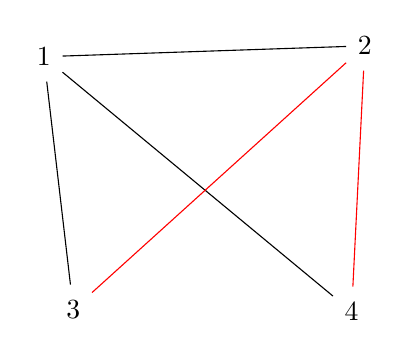
\begin{tikzpicture}[x=0.75pt,y=0.75pt,yscale=-1,xscale=1]
			\draw (237.42,54.74) node   {$1$};
			\draw (392.08,49.49) node   {$2$};
			\draw (251.65,176.51) node   {$3$};
			\draw (385.73,177.51) node   {$4$};
			\draw    (246.42,62.19) -- (376.73,170.06) ;
			\draw    (246.42,54.43) -- (383.08,49.8) ;
			\draw [color={rgb, 255:red, 255; green, 0; blue, 0 }  ,draw opacity=1 ]   (383.08,57.63) -- (260.65,168.37) ;
			\draw    (238.82,66.74) -- (250.25,164.51) ;
			\draw [color={rgb, 255:red, 255; green, 0; blue, 0 }  ,draw opacity=1 ]   (391.49,61.49) -- (386.32,165.51) ;
		\end{tikzpicture}

	\item 0.9: 
		\\G = (V, E) where 	\\
		V = \{1,2,3,4,5,6\}, E=\{\{1,4\},\{1,5\},\{1,6\},\{2,4\},\{2,5\},\{2,6\},\{3,4\},\{3,5\},\{3,6\}\}
\end{itemize}

\end{document}